\documentclass[conference]{IEEEtran}
\usepackage[T1]{fontenc}
\usepackage[utf8]{inputenc}

\usepackage{fullpage}
\usepackage[french]{babel}
\usepackage{graphicx}

\title{PROJ: DeepVoice}

\author{Rémi Hutin \and Rémy Sun \and Raphael Truffet}

\begin{document}

\maketitle


\begin{figure}[!h]
    \centering
    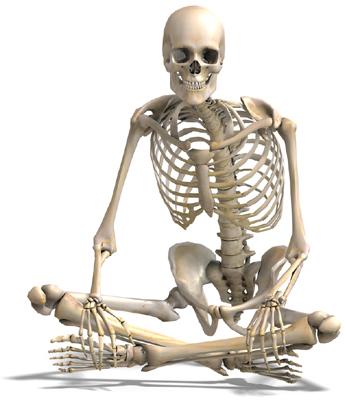
\includegraphics[scale=2]{squelette.jpg}
\end{figure}

\section{Introduction}

\section{Sound signals}

\subsection{Cepstral analysis}

\subsection{GMMs}

\subsection{Supervectors and i-vectors}

\subsection{Previous works}

\section{Use of neuronal networks}

\subsection{Formal neuron}

\paragraph{Neuron?}
A neuron can be thought of as a function which takes an $n$-dimensional vector $A$ as input and returns a scalar $e$ as output. This function typically has two internal parameters which are a bias $b$ and a weight-matrix $W$. The function starts by calculating $WA+b$ before using a non-linear activation function (such as sigmoid or tanh): $e=f(WA+b)$.

\paragraph{Adjusting the function}
Our endgoal is to have the neuron, and by extension the neural network, perform
a certain task. The formal neuron \og learns\fg by adjusting its function to perform better on
this designated task.

For instance, suppose we have a bi-dimensional vector given as input and that we
want our neuron to return 1 if its two coordinates are the identical and -1 if
it is not. A natural way to evaluate how accurate our neuron is by looking at the
distance between its output $e$ and the desired result r : d(e)=|e-r|.

We want to modify our neuron/function to minimize this distance. That means
changing $e$, typically by gradient descent on function $d$ derivative. Here,
$d'(e) = r-e$, which means we want to \og move\fg{} $e$ in this
direction. To this end, we modify our function's two internal parameters $W$ and
$b$. $e$, and by extension can actually be seen as a function of those two
parameters: $d(W,b)=|e(W,b)-r|$. Therefore $\frac{\partial d}{\partial W}
   = \frac{\partial d}{\partial e}\frac{\partial e}{\partial W}$
\paragraph{Neuronal network?}

[Explanation as to the organization in layers and the hierarchical distinctions learned through deep learning]

\subsection{Autoencoders}

An autoencoder is a neuronal network with a particular architecture which is defined below.

\paragraph{A default goal}
Basically, in order to learn a neuronal network, we need to affect to each input of the learning set a label, that is the output we want to enclose, the desired result. However, autoencoders bypass this need by defaulting to an objective that does not require additional information on the input. In fact, the desired result is the input itself.

\paragraph{Structure}
A neuronal network that tries to reconstruct the input may learn the identity. But an autoencoder has a structure the makes it impossible. In fact, an autoencoder has at least one hidden layer that is smaller than the input. So an autoencoder can be decomposed as an encoder that transform the input to a smaller represatation, called latent representation or code, and a decoder that reconstruct the input from the latent representation.

\begin{figure}[!h]
    \centering
    \caption{Structure of an autoencoder}
    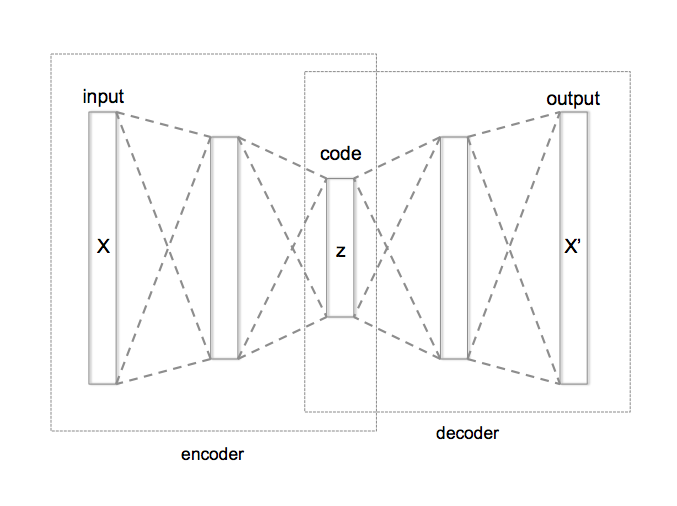
\includegraphics[width=7cm]{Autoencoder_structure.png}
    \label{autoencoder_structure}
\end{figure}


\paragraph{Why use autoencoders?}

Autoencoders can be used for denoising, using corrupted data as input and the original data as objective.

Autoencoders may also be very useful to learn a representation. In fact, the latent represention contains enough information to reconstruct the data.

In our context, autoencoders could be used to find a representation of a speaker, by giving to the autoencoder an i-vector from a speaker as input, and an another i-vector from the same speaker as objective. This idea is based on considerating the withoin-speaker variability as a noise, and using a denoising autoencoder. Repeating this with several pairs of i-vectors, we may learn a representation of the speaker. 



\subsection{Tied weight autoencoder}

\paragraph{Architecture}
[Explanation]

\paragraph{Good results}
[Vedran's paper?]

\section{Method}




\end{document}
